\section{Maxwell-Boltzmann distribution law}
	The Maxwell-Boltzmann distribution is a result of the kinetic theory of gases, which provides a simplified explanation of many fundamental gaseous properties, including pressure and diffusion. This distribution applies fundamentally to particle velocities in three dimensions, but turns out to depend only on the speed (the magnitude of the velocity) of the particles. A particle speed probability distribution indicates which speeds are more likely: a randomly chosen particle will have a speed selected randomly from the distribution, and is more likely to be within one range of speeds than another.
	
	The kinetic theory of gases applies to the classical ideal gas, which is an idealization of real gases. In real gases, there are various effects (e.g., van der Waals interactions, vortical flow, relativistic speed limits, and quantum exchange interactions) that can make their speed distribution different from the Maxwell–Boltzmann form. However, rarefied gases at ordinary temperatures behave very nearly like an ideal gas and the Maxwell speed distribution is an excellent approximation for such gases. This is also true for ideal plasmas, which are ionized gases of sufficiently low density.
	
	\subsection{Postulates of kinetic theory of gases}
		\begin{enumerate}
			\item Every mole of a gas contains about $\num{6.023e23}$ molecules.
			\item The gas molecules may be regarded as point masses.
			\item The gas molecules are in a state of continuous random motion.
			\item In the absence of an external force field, the molecules are distributed uniformly in the container, i.e. an ideal gas behaves as an isotropic medium.
			\item The molecules of a gas experience force only during collisions.
			\item The molecules of a gas behave as rigid, perfectly elastic hard spheres.
			\item The duration of collisions is negligible compared to the time interval between collisions.
			\item There is a spread of molecular speeds from zero to infinity.
			\item The gravitational potential energy has negligible effect on the motion of the gas molecules.
		\end{enumerate}
	
	\subsection{Fundamental assumptions}
		In the derivation of the Maxwell-Boltzmann distribution, we make the following basic assumptions:
		\begin{enumerate}
			\item In the equilibrium state, the molecules have complete randomness of direction and velocity.
			
			\item There is no mass motion or convection current in the body of the gas.
			
			\item The probability of a molecule having an $x$-velocity component at any point of time is independent of its $y$- and $z$-velocity components, and so on.
			
			\item The probability that a molecule selected at random has velocity component in a given range is a function only of the magnitude of the velocity component and the width of the interval.
			
			\item The gas molecules have no rotational or vibrational energies.
		\end{enumerate}
	
	\subsection{Velocity space}
		Consider a gas of $N$ molecules enclosed in a vessel, of arbitrary shape, and moving randomly. The velocity vectors are all randomly oriented in all possible directions.
		\begin{figure}[h!]
			\centering
			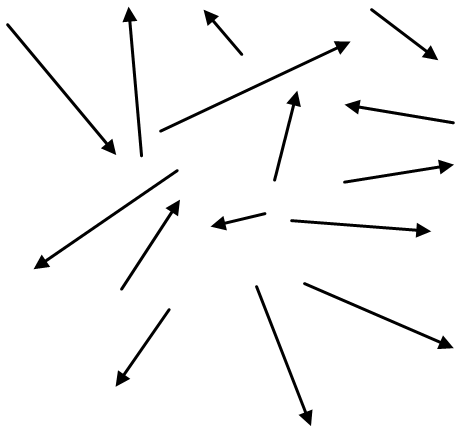
\includegraphics[width=0.45\textwidth]{figures/fig_random-vel.png}
		\end{figure}
		
		Now we transport each vector parallel to itself to a common origin.
		\begin{figure}[h!]
			\centering
			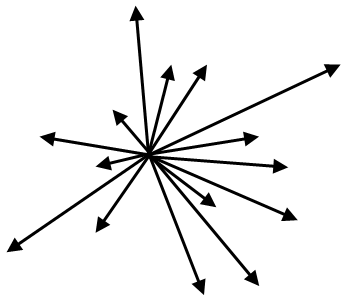
\includegraphics[width=0.35\textwidth]{figures/fig_random-vel-transp.png}
		\end{figure}
		
		If we now fix the velocity axes $v_x$, $v_y$ and $v_z$ with respect to a common origin $O$ (that corresponds to particles at rest), every molecular velocity can be represented in this space, which is known as the \emph{velocity space}.
	
	\subsection{Derivation of Maxwell-Boltzmann distribution law}
		Let us now consider an infinitessimal volume element $\dd{\va*{v}}$ in this velocity space. The number of velocity vectors that terminate inside $\dd{\va*{v}}$ gives us the average number of molecules whose velocities lie between $\va*{v}$ and $\va*{v}+\dd{\va*{v}}$.
		\begin{figure}[h!]
			\centering
			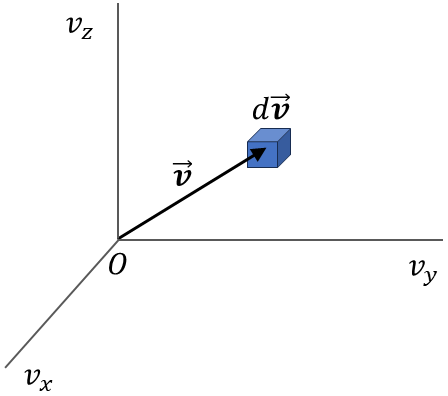
\includegraphics[width=0.35\textwidth]{figures/fig_inf-vel-elem.png}
		\end{figure}
		
		We have, for any velocity $\va*{v}$, the corresponding speed to be
		\begin{align}
			v^2&=v_x^2+v_y^2+v_z^2 \label{eqn:molec-speed-01}
		\end{align}
		Let $\dd{N_{v_x}}$ be the number of molecules having velocity components in the range $v_x$ and $v_x+\dd{v_x}$. Then from assumption \#4, we have
		\begin{align}
			\dfrac{\dd{N_{v_x}}}{N}&=f(v_x)\dd{v_x} \nonumber\\
			\text{or, }\dd{N_{v_x}}&=Nf(v_x)\dd{v_x} \label{eqn:dNvx-01}
		\end{align}
		In equation (\ref{eqn:dNvx-01}), $f(v_x)$ is an unknown function that we have to determine.
		
		Also, the probability of finding a molecule with $x$-velocity component in the range $v_x$ and $v_x+\dd{v_x}$ is
		\begin{align}
			p_x&=\dfrac{\dd{N_{v_x}}}{N}=f(v_x)\dd{v_x} \label{eqn:p_x}
		\end{align}
		
		Likewise, from assumption \#3, we have
		\begin{align}
			p_y&=f(v_y)\dd{v_y} \label{eqn:p_y} \\
			p_z&=f(v_y)\dd{v_z} \label{eqn:p_z}
		\end{align}
		
		Then from the law of compound probabilities, the probability of finding a molecule having velocity components simultaneously in the ranges $[v_x,v_x+\dd{v_x}]$, $[v_y,v_y+\dd{v_y}]$ and $[v_z,v_z+\dd{v_z}]$ is
		\begin{align}
			\dfrac{\dd[3]{N_{v_xv_yv_z}}}{N}&=p_xp_yp_z=f(v_x)f(v_y)f(v_z)\dd{v_x}\dd{v_y}\dd{v_z} \label{eqn:dNv-N}
		\end{align}
		
		Hence, the number density of velocity points is
		\begin{align}
			\rho&=\dfrac{\dd[3]{N_{v_xv_yv_z}}}{\dd{v_x}\dd{v_y}\dd{v_z}}=Nf(v_x)f(v_y)f(v_z) \label{eqn:rho-01}
		\end{align}
		
		It follows from assumption \#1 that the velocity space has been assumed to be isotropic, and so this implies that $\rho$ is independent of the direction of $\va*{v}$ and only depends ton $v^2$, i.e
		\begin{align}
			\rho&\propto J(v^2) \nonumber\\
			\implies f(v_x)f(v_y)f(v_z)&=J(v^2) \label{eqn:J-f}
		\end{align}
		where $J$ is some other function.
		
		For a fixed value of $v^2$, $J(v^2)$ is constant and so
		\begin{align}
			\dd{\qty[J(v^2)]}&=0 \nonumber\\
			\implies\dd{\qty[f(v_x)f(v_y)f(v_z)]}&=0 \nonumber\\
			\implies\pdv{f(v_x)}{v_x}\dd{v_x}f(v_y)f(v_z)+f(v_x)\pdv{f(v_y)}{v_y}\dd{v_y}f(v_z)+f(v_x)f(v_y)\pdv{f(v_z)}{v_z}\dd{v_z}&=0 \label{eqn:diff_f-vxvyvz}
		\end{align}
		
		Dividing equation (\ref{eqn:diff_f-vxvyvz}) by $f(v_x)f(v_y)f(v_z)$, we obtain
		\begin{align}
			\dfrac{1}{f(v_x)}\pdv{f(v_x)}{v_x}\dd{v_x}+\dfrac{1}{f(v_y)}\pdv{f(v_y)}{v_y}\dd{v_y}+\dfrac{1}{f(v_z)}\pdv{f(v_z)}{v_z}\dd{v_z}&=0 \label{eqn:dd_f-vxvyvz}
		\end{align}
		Also, for a fixed value of $v^2$, we have
		\begin{align}
			\dd{\qty[v^2]}&=0 \nonumber\\
			\implies\dd{\qty[v_x^2+v_y^2+v_z^2]}&=0 \nonumber\\
			\implies v_x\dd{v_x}+v_y\dd{v_y}+v_z\dd{v_z}&=0 \label{eqn:v-dv}
		\end{align}
		
		Suppose that $B$ is some unknown constant. Then multiplying equation (\ref{eqn:v-dv}) with $2B$ and adding to equation (\ref{eqn:dd_f-vxvyvz}) gives
		\begin{align}
			\qty[\dfrac{1}{f(v_x)}\pdv{f(v_x)}{v_x}+2Bv_x]\dd{v_x} +  \qty[\dfrac{1}{f(v_y)}\pdv{f(v_y)}{v_y}+2Bv_y]\dd{v_y} +  \qty[\dfrac{1}{f(v_z)}\pdv{f(v_z)}{v_z}+2Bv_z]\dd{v_z} &= 0 \label{eqn:combo-10-11}
		\end{align}
		
		Even though $v$ is held constant, $v_x$, $v_y$, $v_z$ may individually change and yet satisfy equation (\ref{eqn:molec-speed-01}). In equation (\ref{eqn:combo-10-11}), the first term within brackets depends only on $v_x$, the second term on $v_y$ and the third term on $v_z$.
		
		Because $\dd{v_x}$, $\dd{v_y}$, $\dd{v_z}$ are arbitrary, the only way for equation (\ref{eqn:combo-10-11}) to hold good is if all three terms vanish identically.
		
		Therefore, for the $v_x$ term, we would have
		\begin{align*}
			\dfrac{1}{f(v_x)}\pdv{f(v_x)}{v_x}+2Bv_x&=0 \\
			\implies\pdv{f(v_x)}{v_x}&=-2Bv_xf(v_x) \\
			\implies\dfrac{\partial f(v_x)}{f(v_x)}&=-2Bv_x\partial v_x \\
			\implies\int{\dfrac{\dd{f}}{f}}&=-2B\int{v_x\dd{v_x}} \\
			\implies\ln{f(v_x)}&=-2B\dfrac{v_x^2}{2}+\ln{A}
		\end{align*}
		where $\ln{A}$ is the constant of integration. From the above we obtain
		\begin{align}
			\ln{f(v_x)}-\ln{A}&=-Bv_x^2 \nonumber\\
			\implies\ln{\dfrac{f(v_x)}{A}}&=-Bv_x^2 \nonumber\\
			\implies\dfrac{f(v_x)}{A}&=e^{-Bv_x^2} \nonumber\\
			\implies f(v_x)&=Ae^{-Bv_x^2} \label{eqn:fv_x}
		\end{align}
		
		Likewise, from the $v_y$ and $v_z$ terms, we obtain
		\begin{align}
			f(v_y)&=Ae^{-Bv_y^2} \label{eqn:fv_y}\\
			f(v_z)&=Ae^{-Bv_z^2} \label{eqn:fv_z}
		\end{align}
		
		Using equations (\ref{eqn:fv_x}), (\ref{eqn:fv_y}) and (\ref{eqn:fv_z}) in equation (\ref{eqn:rho-01}) gives us
		\begin{align}
			\rho&=N\qty(Ae^{-Bv_x^2})\qty(Ae^{-Bv_y^2})\qty(Ae^{-Bv_z^2}) \nonumber\\
				&=NA^3e^{-B(v_x^2+v_y^2+v_z^2)} \nonumber\\
			\implies\Aboxed{\rho(v)&=NA^3e^{-Bv^2}} \label{eqn:maxwell-vel-distn-01}
		\end{align}
		Equation (\ref{eqn:maxwell-vel-distn-01}) is known as \emph{Maxwell's velocity density distribution function}, where $\rho$ varies with molecular speeds $v$ as shown in the plot below:
		\begin{figure}[h!]
			\centering
			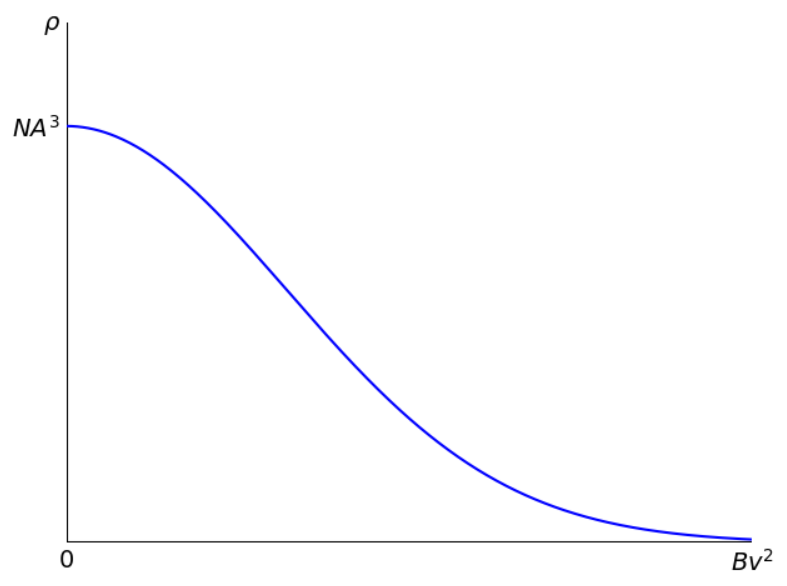
\includegraphics[width=0.65\textwidth]{figures/fig_max-vel-dens-distn.png}
		\end{figure}
	
		\newpage
		\subsubsection{Molecular distribution of speeds}
			\setcounter{equation}{0}
			Consider a spherical shell of radius $v$ and thickness $\dd{v}$ in the velocity space. Then all points within this shell correspond to molecules with speeds in the range $v$ and $v+\dd{v}$.
			\begin{figure}[h!]
				\centering
				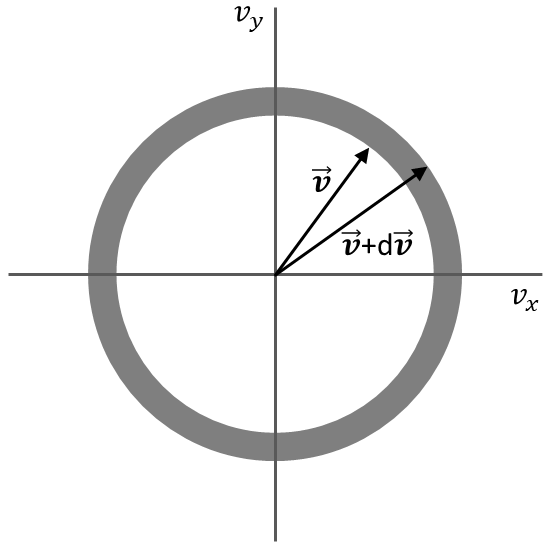
\includegraphics[width=0.45\textwidth]{figures/fig_vel-sph-shell.png}
			\end{figure}
			In the spherical polar coordinates, the volume of an arbitrary volume element is
			\begin{align}
				\dd{v_x}\dd{v_y}\dd{v_z}&=v^2\sin{\theta}\dd{\theta}\dd{\phi}\dd{v} \label{eqn:v-space:vol-elem}
			\end{align}
			The number of molecules with speeds in the range $v$ and $v+\dd{v}$ is obtained by integrating $\rho$ over this shell as
			\begin{align}
				\dd{N_v}&=\dd[3]{N_{v_xv_yv_z}} \nonumber\\
					&=\int\limits_{\theta=0}^{\pi}\int\limits_{\phi=0}^{2\pi}{NA^3e^{-Bv^2}v^2\sin{\theta}\dd{\theta}\dd{\phi}\dd{v}} \nonumber\\
					&=NA^3e^{-Bv^2}v^2\dd{v}\int\limits_{0}^{\pi}{\sin{\theta}\dd{\theta}}\int\limits_{0}^{2\pi}{\dd{\phi}} \nonumber\\
					&=NA^3e^{-Bv^2}v^2\dd{v}\qty[\cos{0}-\cos{\pi}]2\pi \nonumber\\
					&=NA^3e^{-Bv^2}v^2\dd{v}\times 2\times 2\pi \nonumber\\
				\implies\dd{N_v}&=4\pi NA^3v^2e^{-Bv^2}\dd{v} \nonumber \\
				\implies\Aboxed{\dv{N_v}{v}&=4\pi NA^3v^2e^{-Bv^2}} \label{eqn:dNv-dv}
			\end{align}
			Equation (\ref{eqn:dNv-dv}) gives us the \emph{Maxwellian distribution function of molecular speeds}.
			
			\newpage
			\begin{figure}[h!]
				\centering
				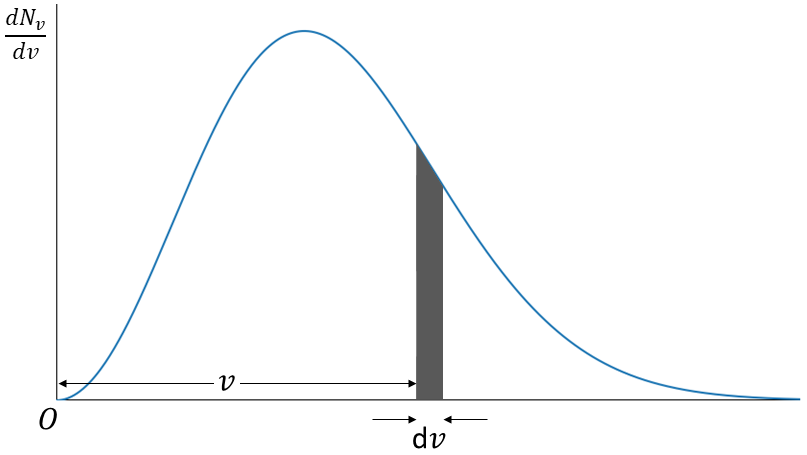
\includegraphics[width=0.7\textwidth]{figures/fig_max-mol-speed-distn.png}
			\end{figure}
			In the plot of $\dv{N_v}{v}$ with respect to $v$, the area of a vertical shaded strip under the graph gives the number of molecules which have speeds between $v$ and $v+\dd{v}$. Hence, the total area under the entire curve gives us the total number of molecules $N$.
	
		\subsubsection{Determination of the constants}
			\setcounter{equation}{0}
			The total number of molecules $N$ can be obtained by integrating $\dd{N_v}$ over all speeds, i.e.
			\begin{align}
				N&=\int{\dd{N_v}}=4\pi NA^3\int\limits_{0}^{\infty}{v^2e^{-Bv^2}\dd{v}} \label{eqn:total-molec-N}
			\end{align}
			
			We now use the following standard integral:
			\begin{align}
				\int\limits_{0}^{\infty}{e^{-\alpha x^2}x^n\dd{x}}&=\dfrac{1}{2\alpha^{(n+1)/2}}\Gamma\qty(\dfrac{n+1}{2}) \label{eqn:std-integ}
			\end{align}
			where the gamma function is defined as
			\begin{align*}
				\Gamma(x)=\int\limits_{0}^{\infty}{t^{x-1}e^{-t}\dd{t}}
			\end{align*}
			
			Some important values of $\Gamma(x)$ are given below:
			\begin{table}[h!]
				\centering
				\begin{tabular}{cc}
					\toprule[1.5pt]
					{$\boldsymbol{x}$} & {$\boldsymbol{\Gamma(x)}$} \\
					\midrule
					{$1/2$} & {$\sqrt{\pi}$} \\
					{$1$} & {$1$} \\
					{$3/2$} & {$\sqrt{\pi}/2$} \\
					{$2$} & {$1$} \\
					\bottomrule[1.5pt]
				\end{tabular}
			\end{table}
			
			The gamma function also satisfies the recurrence relation: $\Gamma(n+1)=n\Gamma(n)$
			
			In equation (\ref{eqn:std-integ}), setting $x\to v$, $\alpha\to B$ and $n=2$ gives us
			\begin{align}
				\int\limits_{0}^{\infty}{e^{-Bv^2}v^2\dd{v}}&=\dfrac{1}{2B^{(2+1)/2}}\Gamma\qty(\dfrac{2+1}{2}) \nonumber\\
					&=\dfrac{1}{2B^{3/2}}\Gamma\qty(\dfrac{3}{2}) \nonumber\\
				\implies\int\limits_{0}^{\infty}{v^2e^{-Bv^2}\dd{v}}&=\dfrac{\sqrt{\pi}}{4B^{3/2}} \label{eqn:integ-in-N}
			\end{align}
			
			Inserting equation (\ref{eqn:integ-in-N}) in equation (\ref{eqn:total-molec-N}), we get
			\begin{align}
				\cancel{N}&=\cancel{4}\pi \cancel{N}A^3\times\dfrac{\sqrt{\pi}}{\cancel{4}B^{3/2}} \nonumber\\
				\implies B^{3/2}&=\sqrt{\pi^3}A^3 \nonumber\\
				\implies A^3&=\dfrac{B^{3/2}}{\sqrt{\pi^3}}=\dfrac{B^{3/2}}{\pi^{3/2}}=\qty(\sqrt{\dfrac{B}{\pi}})^3 \nonumber\\
				\implies A&=\sqrt{\dfrac{B}{\pi}} \label{eqn:const-A-using-B}
			\end{align}
			
			However, equation (\ref{eqn:const-A-using-B}) only gives us the constant $A$ in terms of another constant $B$. We can find $B$ using the law of equipartition of energy of a gas.
			
			The average value of $v^2$ is obtained as
			\begin{align}
				\expval{v^2}&=\dfrac{\int_{0}^{\infty}{v^2\dd{N_v}}}{\int_{0}^{\infty}{\dd{N_v}}} \label{eqn:avg-v2}
			\end{align}
			
			Now, we have
			\begin{align*}
				\int\limits_{0}^{\infty}{v^2\dd{N_v}}&=4\pi NA^3\int\limits_{0}^{\infty}{v^4e^{-Bv^2}\dd{v}} \\
					&=4\pi NA^3\dfrac{\Gamma(5/2)}{2B^{5/2}}\qq{[using the standard integral]} \\
				\implies\int\limits_{0}^{\infty}{v^2\dd{N_v}}&=\dfrac{2\pi NA^3}{B^{5/2}}\Gamma\qty(\dfrac{5}{2})
			\end{align*}
			
			Also, we have
			\begin{align*}
				\int\limits_{0}^{\infty}{\dd{N_v}}&=4\pi NA^3\int\limits_{0}^{\infty}{v^2e^{-Bv^2}\dd{v}}=\dfrac{2\pi NA^3}{B^{3/2}}\Gamma\qty(\dfrac{3}{2})
			\end{align*}
			
			Using the above two integrals in equation (\ref{eqn:avg-v2}), we obtain
			\begin{align}
				\expval{v^2}&=\dfrac{\cancel{2\pi NA^3}\Gamma(5/2)}{B^{5/2}}\cdot\dfrac{B^{3/2}}{\cancel{2\pi NA^3}\Gamma(3/2)} \nonumber\\
					&=\dfrac{B^{3/2}}{B^{5/2}}\cdot\dfrac{\Gamma(5/2)}{\Gamma(3/2)} \nonumber\\
					&=\dfrac{B^{3/2}}{B^{5/2}}\cdot\dfrac{\sfrac{3}{2}\cancel{\Gamma(3/2)}}{\cancel{\Gamma(3/2)}} \nonumber\\
					&=\dfrac{3}{2}B^{\sfrac{3}{2}-\sfrac{5}{2}}=\dfrac{3}{2}B^{-1} \nonumber\\
				\implies\expval{v^2}&=\dfrac{3}{2B} \label{eqn:avg-v2-using-B}
			\end{align}
			
			Hence, the average kinetic energy of the gas molecules becomes
			\begin{align}
				\expval{K}&=\dfrac{1}{2}m\expval{v^2}=\dfrac{1}{2}m\times\dfrac{3}{2B} \nonumber\\
				\implies\expval{K}&=\dfrac{3m}{4B} \label{eqn:avg-K}
			\end{align}
			
			However, from the law of equipartition of energy of a gas, the average kinetic energy of the gas molecules at temperature $T$ is
			\begin{align}
				\expval{K}&=\dfrac{3}{2}k_BT \label{eqn:equipart-law}
			\end{align}
			where $k_B=\num{1.381e-23}\,\unit{\joule\per\kelvin}$ is the Boltzmann constant.
			
			Comparing equations (\ref{eqn:avg-K}) and (\ref{eqn:equipart-law}) gives us
			\begin{align}
				\dfrac{3m}{4B}&=\dfrac{3}{2}k_BT \nonumber\\
				\implies\dfrac{\cancel{3}m}{\cancelto{2}{4}B}&=\dfrac{\cancel{3}}{\cancel{2}}k_BT \nonumber\\
				\implies B&=\dfrac{m}{2k_BT} \label{eqn:const-B}
			\end{align}
			
			Inserting equation (\ref{eqn:const-B}) in equation (\ref{eqn:const-A-using-B}) gives us the value of the constant $A$:
			\begin{align}
				A&=\sqrt{\dfrac{B}{\pi}} \nonumber\\
				\implies A&=\sqrt{\dfrac{m}{2\pi k_BT}} \label{eqn:const-A}
			\end{align}
			
			Finally, substituting for the constants $A$ and $B$ using equations (\ref{eqn:const-A}) and (\ref{eqn:const-B}) respectively in the Maxwellian distribution function for molecular speeds, we get
			\begin{align}
				\dd{N_v}&=4\pi N\qty(\dfrac{m}{2\pi k_BT})^{3/2}v^2e^{-mv^2/2k_BT}\dd{v} \nonumber\\
				\implies\Aboxed{f_v=\dfrac{\dd{N_v}}{N\dd{v}}&=4\pi\qty(\dfrac{m}{2\pi k_BT})^{3/2}v^2e^{-mv^2/2k_BT}} \label{eqn:Maxwell-distn:fv}
			\end{align}
			
			The \emph{Maxwellian density function} $f_v$, from equation (\ref{eqn:Maxwell-distn:fv}), gives us the probability per unit molecular speed of finding a molecule with speed between $v$ and $v+\dd{v}$. This function has the following features:
			\begin{enumerate}
				\item $f_v=0$ for $v=0$ (due to $v^2$) and $f_v\to 0$ for $v\to\infty$ (due to $e^{-mv^2/2k_BT}$).
				
				\item For small molecular speeds, the $v^2$ factor dominates and $f_v$ increases quadratically.
				
				\item As the speed increases, the $e^{-mv^2/2k_BT}$ factor begins to dominate and the distribution starts decaying exponentially after attaining a maximum value.
				
				\begin{figure}[h!]
					\centering
					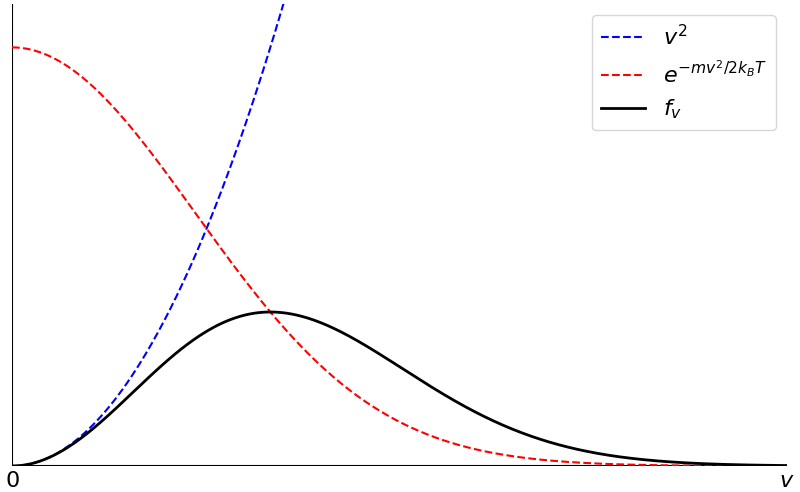
\includegraphics[width=0.9\textwidth]{figures/fig_max-dom-factors.png}
				\end{figure}
				
				\item Because $f_v$ is a probability density function, at all $T$ the following condition must hold good:
				\begin{align*}
					\int\limits_{0}^{\infty}{f_v\dd{v}}=1
				\end{align*}
				
				\item As the temperature $T$ increases, more and more molecules gain kinetic energy and so the peak shifts towards higher molecular speeds. But the total number of molecules remains constant, and so to keep the corresponding area under the curve constant, curve becomes progressively flatter with increasing $T$.
				\newpage
				\begin{figure}[h!]
					\centering
					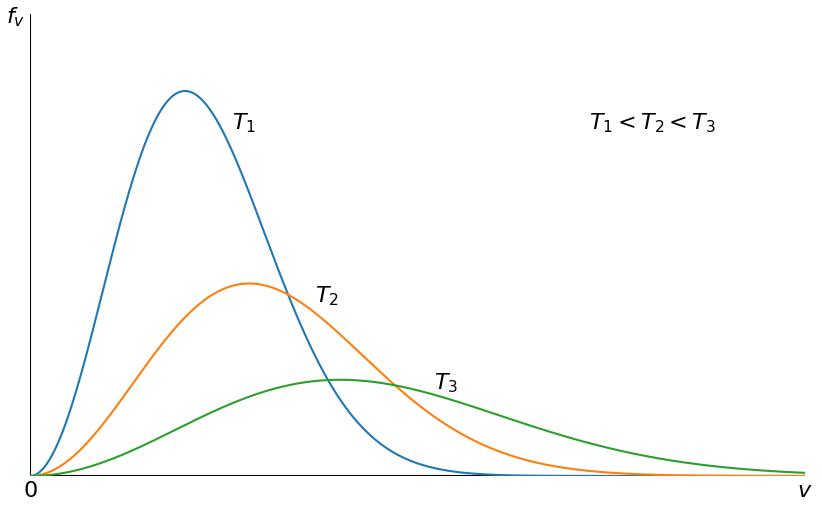
\includegraphics[width=0.9\textwidth]{figures/fig_max-distn-diff-T.png}
				\end{figure}
			\end{enumerate}
			
	\subsection*{Exercises}
		\begin{enumerate}
			\item Calculate the probability that the speed of an \ce{O2} molecule will lie between $100$ m/s and $101$ m/s at $200$ K. The mass of an \ce{O2} molecule is $32$ u. Take $k_B=\num{1.381e-23}\,\unit{\joule\per\kelvin}$ and $N_A=\num{6.023e26}\,\unit{\per\kilo\mole}$.
			
			\item A gas composed of $\num{e6}$ carbon atoms has a Maxwellian velocity distribution at $T=300\,\unit{\kelvin}$. Determine the number of atoms having velocities between\vspace{-1.5ex}
			\begin{enumerate}[(a)]
				\item $100\,\unit{\metre\per\second}$ and $101\,\unit{\metre\per\second}$
				\item $300\,\unit{\metre\per\second}$ and $301\,\unit{\metre\per\second}$
				\item $1500\,\unit{\metre\per\second}$ and $1501\,\unit{\metre\per\second}$
			\end{enumerate}
		\end{enumerate}